\documentclass[aspectratio=169, table]{beamer}

%\usepackage[beamertheme=./praditatheme]{Pradita}
\usepackage[utf8]{inputenc}
\usepackage{xcolor} % for color
\usepackage{colortbl} % for table color
\usepackage{listings}

% Define Java language style for listings
\lstdefinestyle{JavaStyle}{
language=Java,
basicstyle=\ttfamily\scriptsize,
keywordstyle=\color{blue},
commentstyle=\color{gray},
stringstyle=\color{red},
breaklines=true,
showstringspaces=false,
tabsize=2,
captionpos=b,
numbers=left,
numberstyle=\tiny\color{gray},
frame=lines,
backgroundcolor=\color{lightgray!10},
comment=[l]{//},
morecomment=[s]{/*}{*/},
commentstyle=\color{gray}\ttfamily,
string=[s]{'}{'},
morestring=[s]{"}{"},
%	stringstyle=\color{teal}\ttfamily,
%	showstringspaces=false
}

\usetheme{Pradita}
%
\subtitle{IF220303 - Object-oriented Programming}

\title{\Huge{Creational Patterns 2}\\\vspace{30pt}}
\date[Serial]{\scriptsize {PRU/SPMI/FR-BM-18/0222}}
\author[Pradita]{\small {\textbf{Alfa Yohannis}}}

\begin{document}

\frame{\titlepage}

\begin{frame}[fragile]
\frametitle{Contents}
\vspace{20pt}
\begin{columns}[t]
\column{0.5\textwidth}
\tableofcontents[sections={1-2}]

\column{0.5\textwidth}
\tableofcontents[sections={3-4}]
\end{columns}
\end{frame}

\section{Creational Pattern: Builder}

\subsection{Purpose and Context}

\begin{frame}[fragile]{Builder Pattern: Purpose and Context}
\vspace{20pt}
The \textit{Builder} pattern separates the construction of a complex object from its representation.

\vspace{10pt}
\textbf{Builder is useful when:}
\begin{itemize}
\item Objects have many optional attributes or configurations.
\item Object creation requires a specific sequence of steps.
\item Construction logic must be separated from the final product.
\end{itemize}

\vspace{10pt}
\textbf{Typical use cases:}
\begin{itemize}
\item Building structured documents (e.g., PDF, HTML).
\item Creating complex configuration objects (e.g., \texttt{HttpRequest}).
\end{itemize}
\end{frame}

\subsection{Usage Examples}

\begin{frame}[fragile]{Builder Pattern: Usage Examples}
\vspace{20pt}
\textbf{Builder examples:}
\begin{itemize}
\item Constructing a \texttt{Meal} in a fast-food order system.
\item Assembling documents with title, header, body, footer.
\item Building HTTP requests with optional parameters.
\end{itemize}

\vspace{10pt}
\textbf{Real-world practices:}
\begin{itemize}
\item \texttt{StringBuilder} for step-by-step string creation.
\item \texttt{Jackson}, \texttt{Gson} for JSON object builders.
\item UI builders for complex screen layouts (buttons, forms, tables).
\end{itemize}
\end{frame}

\subsection{Advantages and Drawbacks}

\begin{frame}[fragile]{Builder Pattern: Advantages and Drawbacks}
\vspace{20pt}
\textbf{Advantages:}
\begin{itemize}
\item Manages complex object creation step by step.
\item Supports the \textit{Single Responsibility Principle}.
\item Enables method chaining (\texttt{builder.setA().setB()}).
\item Improves flexibility and code readability.
\end{itemize}

\vspace{10pt}
\textbf{Drawbacks:}
\begin{itemize}
\item Increases the number of classes.
\item Overkill for simple objects.
\item Risk of method call order mistakes.
\end{itemize}
\end{frame}

\subsection{Implementation in Java}

\begin{frame}[fragile]{Builder Pattern in Java: Overview}
\vspace{20pt}
The Builder pattern separates the object construction process from its final representation.

\begin{figure}[h]
\centering
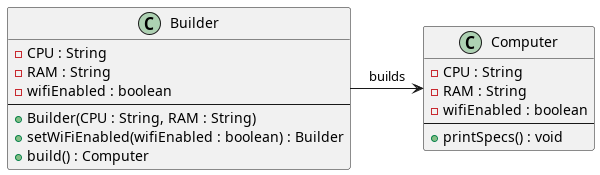
\includegraphics[width=.9\textwidth]{../../figures/out/builder.png}
\caption{Builder Pattern Structure}
\label{fig:builder}
\end{figure}
\end{frame}

\begin{frame}[fragile]{Builder Pattern in Java: Computer Class}
\vspace{30pt}
The Computer class uses a static Builder class to assemble its fields step-by-step.

\begin{columns}[T]
\column{0.5\textwidth}
\begin{lstlisting}[style=JavaStyle]
	public class Computer {
		private String CPU;
		private String RAM;
		private String storage;
		
		private Computer(Builder builder) {
			this.CPU = builder.CPU;
			this.RAM = builder.RAM;
			this.storage = builder.storage;
		}
		
		public void printSpecs() {
			System.out.println("CPU: " + CPU);
			System.out.println("RAM: " + RAM);
			System.out.println("Storage: " + storage);
		}
	\end{lstlisting}
	
	\column{0.5\textwidth}
	\begin{lstlisting}[style=JavaStyle]
		public static class Builder {
			private String CPU;
			private String RAM;
			private String storage;
			public Builder(String CPU, String RAM) {
				this.CPU = CPU;
				this.RAM = RAM;
			}
			public Builder setStorage(String storage) {
				this.storage = storage;
				return this;
			}
			public Computer build() {
				return new Computer(this);
			}
		}
	}
\end{lstlisting}
\end{columns}
\end{frame}


\begin{frame}[fragile]{Builder Pattern in Java: Usage Example}
\vspace{20pt}
Clients can flexibly build Computer objects using chained method calls.

\begin{lstlisting}[style=JavaStyle]
public class Main {
	public static void main(String[] args) {
		Computer pc1 = new Computer.Builder("Intel i5", "8GB")
		.setStorage("512GB SSD")
		.build();
		
		pc1.printSpecs();
		
		Computer pc2 = new Computer.Builder("AMD Ryzen 5", "16GB")
		.build();
		
		pc2.printSpecs();
	}
}
\end{lstlisting}
\end{frame}

\begin{frame}[fragile]{Builder Pattern in Java: TicketOrder Class}
\vspace{30pt}
The TicketOrder class uses a static Builder to configure mandatory and optional fields.

\begin{columns}[T]
\column{0.5\textwidth}
\begin{lstlisting}[style=JavaStyle, basicstyle=\ttfamily\tiny]
	public class TicketOrder {
		private String eventName;
		private String seatNumber;
		private boolean withMeal;
		
		private TicketOrder(Builder builder) {
			this.eventName = builder.eventName;
			this.seatNumber = builder.seatNumber;
			this.withMeal = builder.withMeal;
		}
		
		public void printOrder() {
			System.out.println("Event: " + eventName);
			System.out.println("Seat: " + seatNumber);
			System.out.println("Meal Included: " + withMeal);
		}
	\end{lstlisting}
	
	\column{0.5\textwidth}
	\begin{lstlisting}[style=JavaStyle, basicstyle=\ttfamily\tiny]
		public static class Builder {
			private String eventName;
			private String seatNumber;
			private boolean withMeal = false;
			
			public Builder(String eventName, String seatNumber) {
				this.eventName = eventName;
				this.seatNumber = seatNumber;
			}
			
			public Builder setWithMeal(boolean withMeal) {
				this.withMeal = withMeal;
				return this;
			}
			
			public TicketOrder build() {
				return new TicketOrder(this);
			}
		}
	}
\end{lstlisting}
\end{columns}
\end{frame}

\begin{frame}[fragile]{Builder Pattern in Java: TicketOrder Usage}
\vspace{20pt}
Clients flexibly build TicketOrder objects with optional settings.

\begin{lstlisting}[style=JavaStyle]
public class Main {
	public static void main(String[] args) {
		TicketOrder order1 = new TicketOrder.Builder("Concert A", "A12")
		.setWithMeal(true)
		.build();
		
		order1.printOrder();
		
		TicketOrder order2 = new TicketOrder.Builder("Theatre B", "B25")
		.build();
		
		order2.printOrder();
	}
}
\end{lstlisting}
\end{frame}

\section{Creational Pattern: Prototype}

\subsection{Purpose and Context}

\begin{frame}[fragile]{Prototype Pattern: Purpose and Context}
	\vspace{20pt}
	The Prototype pattern allows creating new objects by copying existing ones instead of building from scratch.
	
	\vspace{10pt}
	\textbf{Main goals:}
	\begin{itemize}
		\item Reduce the cost of creating complex objects.
		\item Simplify object creation by cloning predefined templates.
		\item Allow flexibility to create variations without depending on concrete classes.
	\end{itemize}
	
	\vspace{5pt}
	\textbf{Cloning strategies:}
	\begin{itemize}
		\item \textbf{Shallow Copy}: Copies primitive fields; references remain shared.
		\item \textbf{Deep Copy}: Recursively clones referenced objects to achieve full independence.
	\end{itemize}
\end{frame}

\subsection{Example Use Cases}

\begin{frame}[fragile]{Prototype Pattern: Example Use Cases}
	\vspace{20pt}
	The Prototype pattern is widely used for fast object replication with minor customisations.
	
	\vspace{10pt}
	\textbf{Typical applications:}
	\begin{itemize}
		\item Game character creation from base templates like \texttt{Warrior}, \texttt{Mage}.
		\item Graphic design tools cloning shapes, icons, and UI elements.
		\item Document management systems duplicating report templates.
		\item Configuration systems creating user-specific settings from a default configuration.
	\end{itemize}
	
	\vspace{5pt}
	This pattern ensures efficiency and consistency across objects with similar structures.
\end{frame}

\subsection{Advantages and Drawbacks}

\begin{frame}[fragile]{Prototype Pattern: Advantages and Drawbacks}
	\vspace{20pt}
	The Prototype pattern offers major benefits, but also some challenges in complex systems.
	
	\vspace{10pt}
	\begin{columns}[T]
		\column{0.48\textwidth}
		\textbf{Advantages:}
		\begin{itemize}
			\item Faster and cheaper object creation.
			\item Ensures structural consistency.
			\item Enables dynamic object generation at runtime.
			\item Simplifies creating slight variations.
			\item Reduces class coupling in client code.
		\end{itemize}
		
		\column{0.48\textwidth}
		\textbf{Drawbacks:}
		\begin{itemize}
			\item Difficulties in deep cloning implementation.
			\item Risk of shared references with shallow copies.
			\item Some objects are not easily clonable.
			\item Harder debugging due to many similar instances.
			\item High dependency on correct \texttt{clone()} implementation.
		\end{itemize}
	\end{columns}
\end{frame}


\subsection{Implementation in Java}

\begin{frame}[fragile]{Prototype Pattern in Java: Overview}
	\vspace{20pt}
	The Prototype pattern allows an object to create a copy of itself via the \texttt{clone()} method.
	
	\begin{figure}[h]
		\centering
		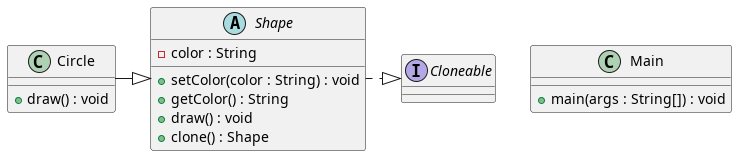
\includegraphics[width=.9\textwidth]{../../figures/out/prototype.png}
		\caption{Prototype Pattern Structure}
		\label{fig:prototype}
	\end{figure}
\end{frame}

\begin{frame}[fragile]{Prototype Pattern in Java: Shape Class}
	\vspace{20pt}
	The Shape abstract class defines cloneable objects with shared colour properties.
	
	\vspace{10pt}
	\begin{columns}[T]
		\column{0.5\textwidth}
		\begin{lstlisting}[style=JavaStyle]
			public abstract class Shape 
			implements Cloneable {
				protected String color;
				
				public void setColor(String color) {
					this.color = color;
				}
				
				public String getColor() {
					return color;
				}
			\end{lstlisting}
			
			\column{0.5\textwidth}
			\begin{lstlisting}[style=JavaStyle, firstnumber=12]
				public abstract void draw();
				
				@Override
				public Shape clone() {
					try {
						return (Shape) super.clone();
					} catch (CloneNotSupportedException e) {
						throw new AssertionError();
					}
				}
			}
		\end{lstlisting}
	\end{columns}
\end{frame}



\begin{frame}[fragile]{Prototype Pattern in Java: Circle Subclass}
	\vspace{20pt}
	The Circle class extends Shape and customises the drawing behaviour.
	
	\vspace{10pt}
	\begin{lstlisting}[style=JavaStyle]
		public class Circle extends Shape {
			@Override
			public void draw() {
				System.out.println(
				"Drawing a " + color + " circle."
				);
			}
		}
	\end{lstlisting}
\end{frame}

\begin{frame}[fragile]{Prototype Pattern in Java: Usage Example}
	\vspace{20pt}
	The client creates a Circle, clones it, modifies the clone, and draws both independently.
	
	\vspace{10pt}
	\begin{lstlisting}[style=JavaStyle]
		public class Main {
			public static void main(String[] args) {
				Circle originalCircle = new Circle();
				originalCircle.setColor("Red");
				
				Circle clonedCircle = 
				(Circle) originalCircle.clone();
				clonedCircle.setColor("Blue");
				
				originalCircle.draw();   
				clonedCircle.draw();     
			}
		}
	\end{lstlisting}
\end{frame}

\begin{frame}[fragile]{Prototype Pattern in Java: Report Class}
\vspace{20pt}
The Report class implements Prototype to enable quick duplication of report documents.

\begin{columns}[T]
\column{0.5\textwidth}
\begin{lstlisting}[style=JavaStyle, firstnumber=1, basicstyle=\ttfamily\tiny]
public class Report implements Cloneable {
	private String title;
	private String content;
	
	public Report(String title, String content) {
		this.title = title;
		this.content = content;
	}
	
	public void setTitle(String title) {
		this.title = title;
	}
	
	public void setContent(String content) {
		this.content = content;
	}
\end{lstlisting}

\column{0.5\textwidth}
\begin{lstlisting}[style=JavaStyle, firstnumber=17, basicstyle=\ttfamily\tiny]
	public void printReport() {
		System.out.println("Title: " + title);
		System.out.println("Content: " + content);
	}
	
	@Override
	public Report clone() {
		try {
			return (Report) super.clone();
		} catch (CloneNotSupportedException e) {
			throw new AssertionError();
		}
	}
}
\end{lstlisting}
\end{columns}
\end{frame}


\begin{frame}[fragile]{Prototype Pattern in Java: Usage Example}
	\vspace{20pt}
	Reports can be cloned and independently modified without affecting the original.
	
	\vspace{10pt}
	\begin{lstlisting}[style=JavaStyle]
		public class Main {
			public static void main(String[] args) {
				Report monthlyReport = 
				new Report("Monthly Report", 
				"Summary of activities...");
				
				Report clonedReport = 
				monthlyReport.clone();
				clonedReport.setTitle(
				"Monthly Report - Copy");
				
				monthlyReport.printReport();
				System.out.println();
				clonedReport.printReport();
			}
		}
	\end{lstlisting}
\end{frame}


\section{Pola Kreasi: Dependency Injection}

\subsection{Purpose and Context}
\begin{frame}[fragile]{Dependency Injection: Purpose and Context}
	\vspace{20pt}
	Dependency Injection (DI) manages object dependencies by injecting them from outside instead of creating them internally.
	
	\textbf{Goals:}
	\begin{itemize}
		\item Reduce tight coupling between classes for flexibility and easier testing.
		\item Enable easier changes and adaptation by replacing dependencies externally.
		\item Support Dependency Inversion Principle (DIP) by depending on abstractions.
	\end{itemize}
	
	\textbf{Injection Methods:}
	\begin{itemize}
		\item \textbf{Constructor Injection}: Inject dependencies via constructor parameters.
		\item \textbf{Setter Injection}: Inject dependencies via setter methods.
		\item \textbf{Interface Injection}: Define dependency injection via an interface method.
	\end{itemize}
	
	Manual or framework-based injection (like Spring) improves modularity and scalability in large systems.
\end{frame}

\subsection{Usage Examples}
\begin{frame}[fragile]{Dependency Injection: Use Cases}
	\vspace{20pt}
	Dependency Injection increases system flexibility in managing service variations and simplifies testing.
	
	\vspace{10pt}
	\textbf{Common Examples:}
	\begin{itemize}
		\item \textbf{Payment Service:} \texttt{OrderService} receives different \texttt{PaymentProcessor} implementations like credit card or PayPal.
		\item \textbf{Logging System:} \texttt{Application} receives different \texttt{Logger} objects without code modification.
		\item \textbf{Unit Testing:} Replace database access with a \texttt{MockDatabase} during tests.
	\end{itemize}
	
	Frameworks like Spring (Java) or Dagger (Android) automate dependency management and injection for large applications.
\end{frame}


\subsection{Advantages and Drawbacks}
\begin{frame}[fragile]{DI: Advantages and Drawbacks}
	\vspace{20pt}
	Dependency Injection provides major design benefits but also adds complexity.
	
	\begin{columns}[T]
		\column{0.5\textwidth}
		\textbf{Advantages:}
		\begin{itemize}
			\item Decouples class relationships for modularity.
			\item Simplifies unit testing with mock objects.
			\item Supports SOLID principles, especially DIP.
			\item Structures and manages complex dependencies.
			\item Increases flexibility and scalability of the system.
		\end{itemize}
		
		\column{0.5\textwidth}
		\textbf{Drawbacks:}
		\begin{itemize}
			\item Adds initial complexity, especially for small projects.
			\item Requires deeper understanding of configuration.
			\item Manual management can be error-prone in large systems.
			\item Increases startup time for complex object graphs.
			\item Introduces dependency on external frameworks.
		\end{itemize}
	\end{columns}
\end{frame}

\subsection{Implementation in Java}
\begin{frame}[fragile]{Dependency Injection in Java: Overview}
	\vspace{20pt}
	Dependency Injection allows objects to receive their dependencies from external sources instead of creating them internally.
	
	\begin{figure}[h]
		\centering
		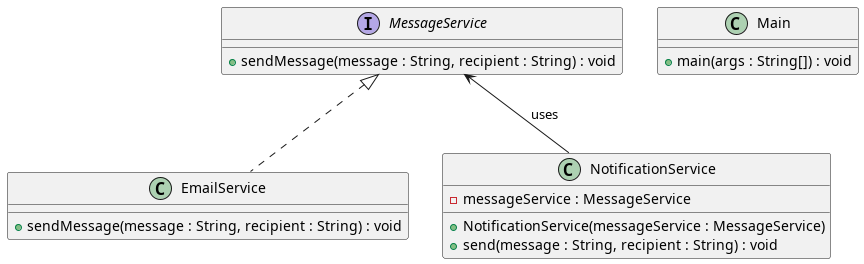
\includegraphics[width=.9\textwidth]{../../figures/out/dependency_injection.png}
		\caption{Dependency Injection Structure}
		\label{fig:dependency-injection}
	\end{figure}
\end{frame}

\begin{frame}[fragile]{Step 1: Defining the Service Interface}
\vspace{20pt}
The MessageService interface defines the contract for sending messages without binding to any specific implementation.

\begin{lstlisting}[style=JavaStyle]
public interface MessageService {
	void sendMessage(String message, String recipient);
}
\end{lstlisting}
\end{frame}

\begin{frame}[fragile]{Step 2: Implementing the Concrete Service}
\vspace{20pt}
The EmailService class implements MessageService and simulates sending an email by printing to the console.

\begin{lstlisting}[style=JavaStyle]
public class EmailService implements MessageService {
	@Override
	public void sendMessage(String message, String recipient) {
		System.out.println("Email sent to " + recipient +
		" with message: " + message);
	}
}
\end{lstlisting}
\end{frame}

\begin{frame}[fragile]{Step 3: Injecting Dependency into Client}
\vspace{20pt}
The NotificationService class receives its MessageService dependency through constructor injection.

\begin{lstlisting}[style=JavaStyle]
public class NotificationService {
	private MessageService messageService;
	
	public NotificationService(MessageService messageService) {
		this.messageService = messageService;
	}
	
	public void send(String message, String recipient) {
		messageService.sendMessage(message, recipient);
	}
}
\end{lstlisting}
\end{frame}

\begin{frame}[fragile]{Step 4: Running the Injection in Main}
\vspace{20pt}
The main method manually injects an EmailService into NotificationService and sends a test message.

\begin{lstlisting}[style=JavaStyle]
public class Main {
	public static void main(String[] args) {
		MessageService service = new EmailService();
		NotificationService notification =
		new NotificationService(service);
		
		notification.send(
		"Hello, Dependency Injection!",
		"user@example.com"
		);
	}
}
\end{lstlisting}
\end{frame}

\begin{frame}[fragile]{Step 1: Defining the Weather Service Interface}
\vspace{20pt}
The WeatherService interface defines the contract for providing weather information independently of its implementation.

\begin{lstlisting}[style=JavaStyle]
public interface WeatherService {
	String getWeatherUpdate();
}
\end{lstlisting}
\end{frame}

\begin{frame}[fragile]{Step 2: Implementing the Weather Service}
\vspace{20pt}
The WeatherAPIService class implements WeatherService and provides a simple weather update.

\begin{lstlisting}[style=JavaStyle]
public class WeatherAPIService implements WeatherService {
	@Override
	public String getWeatherUpdate() {
		return "Today's weather: Sunny, 30 degrees Celsius.";
	}
}
\end{lstlisting}
\end{frame}

\begin{frame}[fragile]{Step 3: Creating the Client with Setter Injection}
\vspace{20pt}
The WeatherReporter client receives its dependency through a setter method, allowing flexibility after instantiation.

\begin{columns}[T]
\column{0.5\textwidth}
\begin{lstlisting}[style=JavaStyle]
public class WeatherReporter {
	private WeatherService weatherService;
	
	public WeatherReporter() {
		// Default constructor
	}
	
	public void setWeatherService(WeatherService weatherService) {
		this.weatherService = weatherService;
	}
\end{lstlisting}

\column{0.5\textwidth}
\begin{lstlisting}[style=JavaStyle, firstnumber=11]
	public void report() {
		if (weatherService != null) {
			System.out.println(weatherService.getWeatherUpdate());
		} else {
			System.out.println("WeatherService is not available.");
		}
	}
}
\end{lstlisting}
\end{columns}
\end{frame}

\begin{frame}[fragile]{Step 4: Running Setter Dependency Injection}
\vspace{20pt}
The main method manually injects WeatherAPIService into WeatherReporter and displays the weather update.

\begin{lstlisting}[style=JavaStyle]
public class Main {
	public static void main(String[] args) {
		WeatherService service = new WeatherAPIService();
		
		WeatherReporter reporter = new WeatherReporter();
		reporter.setWeatherService(service);
		
		reporter.report();
	}
}
\end{lstlisting}
\end{frame}

\section{Conclusions}

\begin{frame}[fragile]{Conclusions}
\vspace{20pt}
This chapter covered three essential creational patterns: \textbf{Builder} for constructing complex objects gradually, \textbf{Prototype} for cloning objects efficiently, and \textbf{Dependency Injection} for managing object dependencies flexibly.

\vspace{10pt}
Using these patterns improves modularity, scalability, readability, and maintainability of software systems, supporting modern design principles like modularity, flexibility, and separation of concerns.
\end{frame}

\end{document}
